\section{实验评估}

\subsection{实验设置}

我们使用第~\ref{sec:implementation} 节描述的部署配置对 EdgeSched 进行评估。为了明确评估标准，我们将结果归纳为五个系统属性：\textbf{可用性}、\textbf{时延退化}、\textbf{恢复时间}、\textbf{吞吐开销}以及\textbf{负载下的完成行为}。这些类别分别对应本文的核心主张：保持常驻服务可达、约束临时降级的代价、可预测地恢复高性能执行、限制调度器成本，并在混合工作负载和故障条件下维持系统可运行。

\textbf{评估指标}：
\begin{itemize}
\item \textbf{可用性}：当突发工作负载占用 GPU 时，常驻服务是否仍然可用。
\item \textbf{时延退化}：迁移与共存期间的 TTFT（Time To First Token）以及可见中断。
\item \textbf{恢复时间}：在工作负载切换或进程故障后恢复服务所需的时间。
\item \textbf{吞吐开销}：相对最小化的信号量实现，系统总体吞吐的下降比例。
\item \textbf{任务成功率}：在混合负载与崩溃场景下，提交任务是否能在未观察到丢失的情况下完成。
\end{itemize}

\textbf{基线设计理由}。我们将 EdgeSched 与若干体现不同设计哲学的实际替代方案进行比较，而不是随意挑选实现。\textbf{冷重启}代表一种\emph{基于重启的设计}，通过杀死并重新加载常驻工作负载来解决冲突。\textbf{操作员管理的手动切换}代表一种\emph{运维人工仲裁设计}，即把资源仲裁移出运行时，通过人工卸载/重载模型来处理。\textbf{OS 级分页/LRU 风格行为}代表一种\emph{不具备应用层工作负载语义的通用内存管理方式}。\textbf{对称迁移}代表一种\emph{统一策略设计}，在两个方向上都采用相同的 stop$\rightarrow$migrate$\rightarrow$resume 逻辑，而不使用 EdgeSched 的 Atomic Hot-Swap 这一不对称优化。仅就开销而言，我们还报告了\textbf{原始信号量实现}，将其作为实现成本参考，而不是完整调度基线。

\subsection{可用性与时延退化}

EdgeSched 的核心能力，是让一个常驻、可迁移的工作负载与一个突发、GPU 绑定的工作负载在单块 8GB GPU 上分时共享，并在抢占期间让常驻工作负载回退到系统内存。在我们的具体实例中，这两类工作负载分别对应 LLM 服务和图像生成。

\subsubsection{迁移时延与共存}

我们测量了一个完整迁移周期中的系统行为：（1）LLM 在 GPU 上运行；（2）图像任务抢占，LLM 卸载到 CPU；（3）图像任务执行；（4）LLM 再迁移回 GPU。表~\ref{tab:migration} 给出了资源迁移性能指标，图~\ref{fig:migration} 则展示了完整迁移时间线，直观呈现了下行（GPU$\rightarrow$CPU）和上行（CPU$\rightarrow$GPU）路径的不对称行为。

\begin{table}[t]
\centering
\caption{Dynamic Resource Migration Results (N=5)}
\label{tab:migration}
\resizebox{\columnwidth}{!}{%
\begin{tabular}{@{}lcc@{}}
\toprule
\textbf{Metric} & \textbf{EdgeSched} & \textbf{Symmetric Migration} \\
\midrule
LLM GPU TTFT (ms) & 112.9 $\pm$ 12.2 & 87.1 $\pm$ 10.4 \\
CPU TTFT (ms) & 200.0 $\pm$ 19.6 & 209.0 $\pm$ 5.7 \\
Downlink Stutter (ms) & 8774.3 $\pm$ 1768.8 & -- \\
\midrule
Restore Time (ms) & 11237.9 $\pm$ 1226.2 & 5728.3 $\pm$ 148.3 \\
Restore Gap (ms) & $\approx$0 & 1308.9 $\pm$ 2415.0 \\
\midrule
Queue Wait Time (ms) & 10024.8 & -- \\
\bottomrule
\end{tabular}%
}
\end{table}


\begin{figure}[!t]
\centering
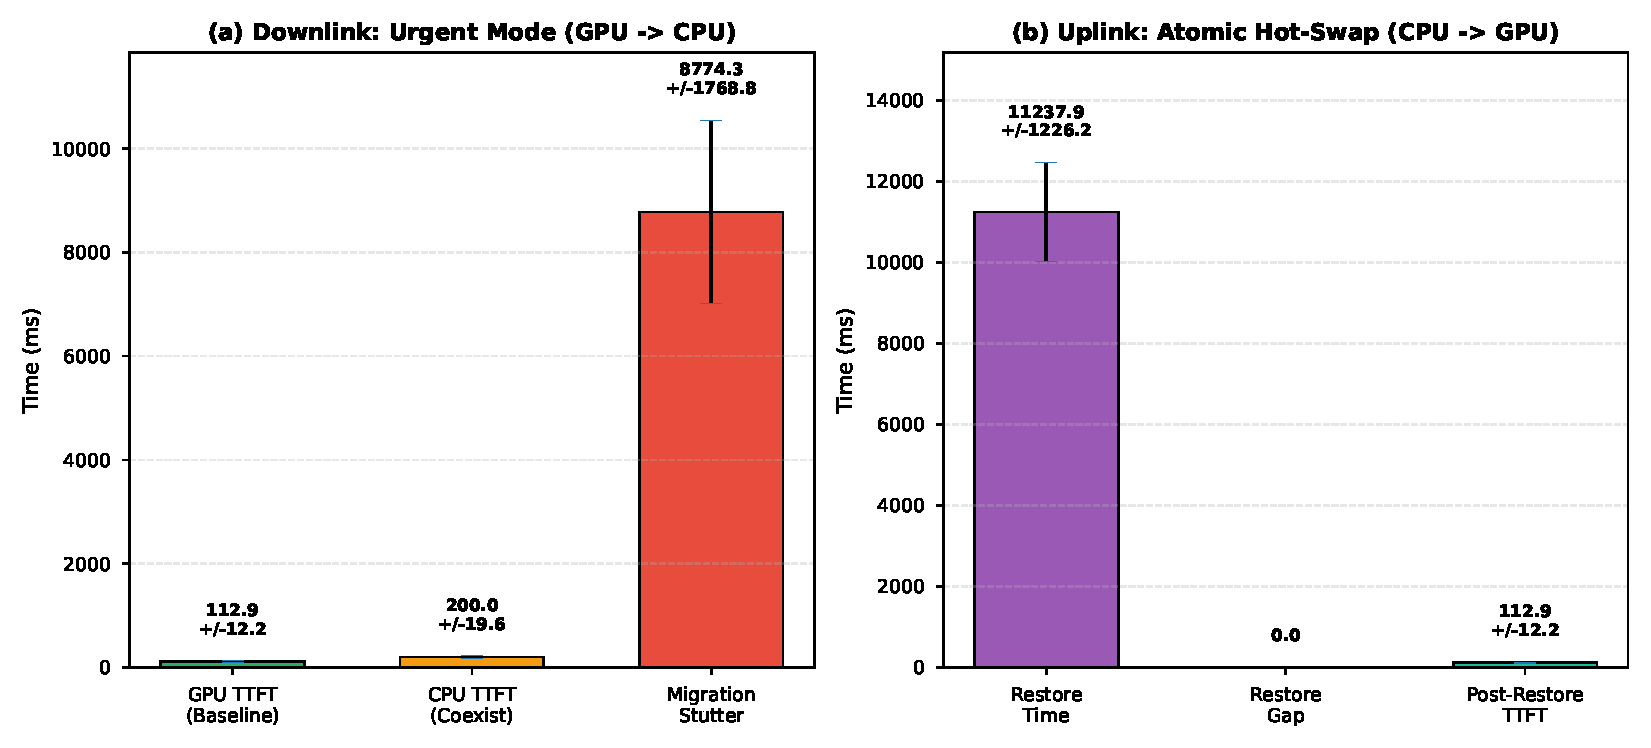
\includegraphics[width=\columnwidth]{figures/01_paper_main/migration/fig_resource_migration.pdf}
\caption{带有 TTFT 测量的迁移时间线。该图展示了下行迁移（Urgent Mode）与上行恢复（Atomic Hot-Swap）的不对称行为。}
\label{fig:migration}
\end{figure}

\textbf{分析}：
\begin{itemize}
\item \textbf{可用性}：常驻工作负载在突发任务执行期间并未完全不可用，而是降级到 CPU 服务后继续保持可达。
\item \textbf{低中断恢复}：在 EdgeSched 中，用户感知到的中断（Restore Gap）接近于零；而对称迁移则表现出更大且波动明显的中断窗口，为 1308.9 $\pm$ 2415.0 ms。这与 \textbf{Atomic Hot-Swap} 的策略一致：CPU 实例在 GPU 实例后台预加载期间继续提供服务。
\item \textbf{时延退化}：在聚合后的迁移实验中，记录到的共存期 TTFT 指标在 EdgeSched 下为 \textbf{200.0 $\pm$ 19.6 ms}，在对称迁移下为 \textbf{209.0 $\pm$ 5.7 ms}（$N=5$）。我们将该日志指标视为调度器侧的信号，而不是用户感知时延的完整刻画，因此还结合图~\ref{fig:real_workload} 中的真实会话轨迹，其中图像执行期间 CPU 阶段请求时延范围为 0.26--8.99 s。
\item \textbf{迁移代价}：EdgeSched 的下行停顿（\textbf{8774.3 $\pm$ 1768.8 ms}）体现了 Urgent Mode 卸载的成本。它的恢复时间（\textbf{11237.9 $\pm$ 1226.2 ms}）比对称迁移的 \textbf{5728.3 $\pm$ 148.3 ms} 更长，但这部分成本大多被后台预加载和接近于零的可见切换中断所隐藏。
\end{itemize}

\subsubsection{队列反压与互斥}

为了验证在突发请求排队时系统仍能保持可用性，我们在活跃的 LLM 会话期间并发提交了多个图像生成任务。

\begin{itemize}
\item \textbf{队列等待时间}：第二个图像任务排在第一个之后等待，而没有触发 OOM，也没有与前一个任务重叠使用 GPU。
\item \textbf{行为}：系统严格执行 GPU 互斥；第二个任务会一直等待到第一个任务完成并释放资源，而不是触发 OOM。
\item \textbf{可用性}：在图像队列处理全过程中，常驻 LLM 服务始终在 CPU 上保持响应。
\end{itemize}

\subsubsection{真实工作负载轨迹}

图~\ref{fig:real_workload} 展示了一个包含 LLM 对话与图像生成的真实交互会话完整时间线。

\begin{figure}[H]
\centering
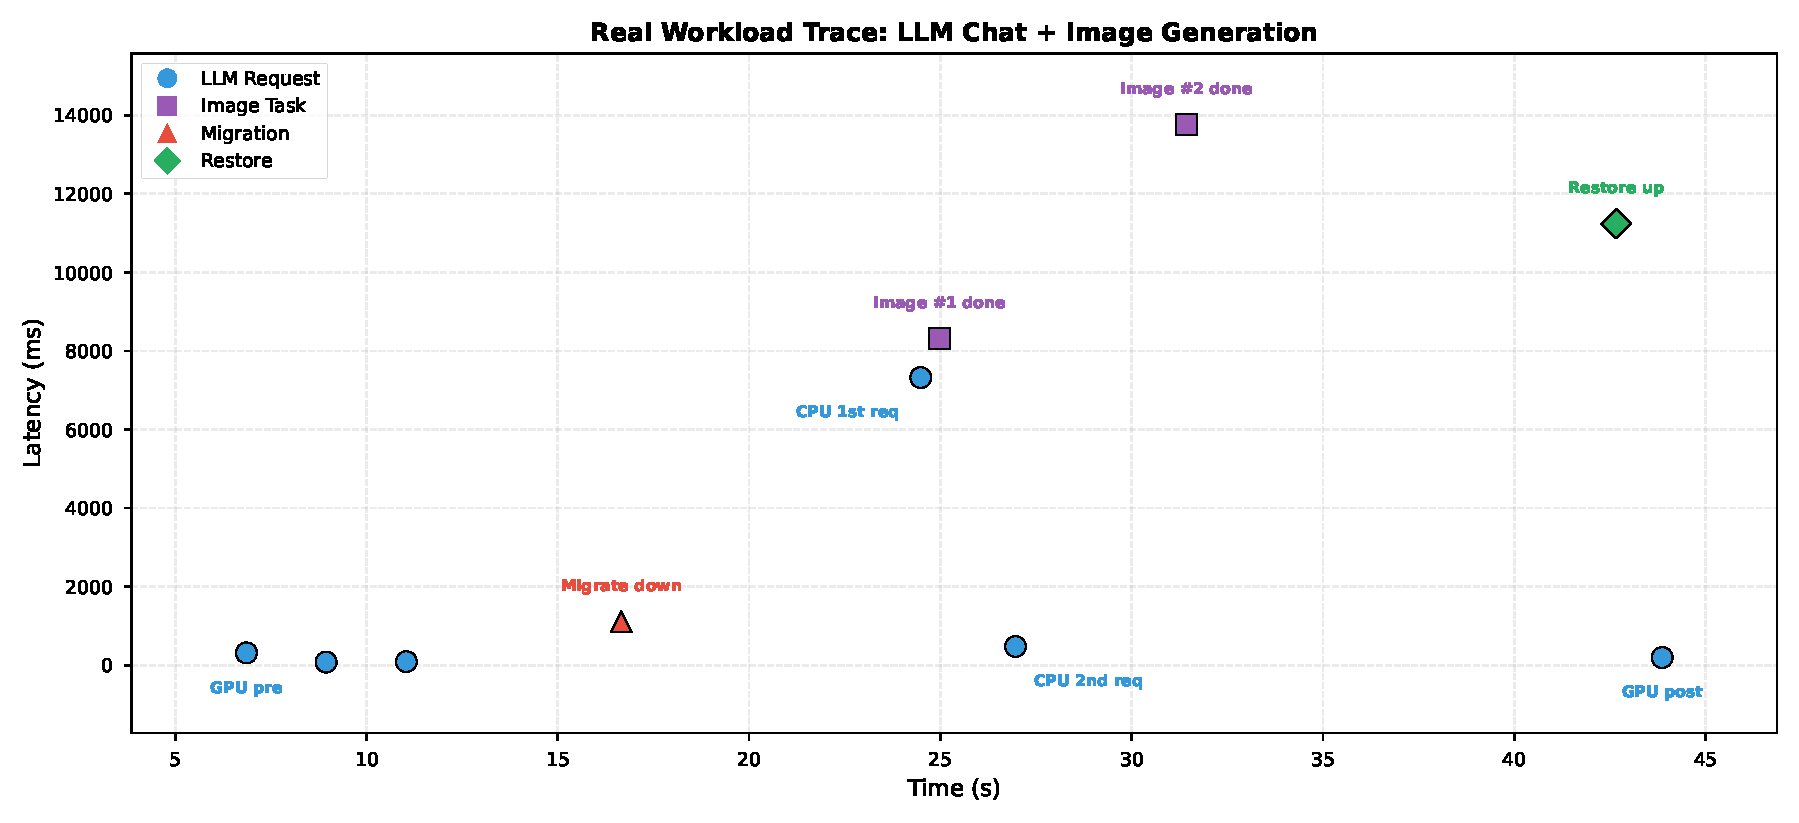
\includegraphics[width=0.96\columnwidth]{figures/02_auxiliary/chart_real_workload_trace.pdf}
\caption{真实工作负载轨迹，展示了重复会话中图像突发前、中、后的 TTFT 变化。图像任务前 GPU TTFT 为 0.04--0.32s；图像执行期间 CPU 阶段请求时延为 0.26--8.99s；恢复后的 GPU TTFT 为 0.20--2.09s。}
\label{fig:real_workload}
\end{figure}

\textbf{观察}：
\begin{itemize}
\item \textbf{GPU 阶段}：TTFT 为 0.04--0.32s，说明在突发任务到来前交互具有良好响应性。
\item \textbf{迁移}：在记录的多个会话中，GPU$\rightarrow$CPU 迁移耗时为 1.01--1.13s。
\item \textbf{共存阶段}：图像生成期间，CPU 阶段请求时延为 0.26--8.99s，但服务始终处于“降级但可用”的状态。
\item \textbf{恢复}：在重复会话轨迹中，CPU$\rightarrow$GPU 恢复耗时为 10.74--11.53s。
\item \textbf{恢复后}：恢复完成后，GPU TTFT 回到 0.20--2.09s。
\end{itemize}

\FloatBarrier

\subsection{恢复时间}

我们从两种形式评估恢复：\textbf{服务恢复}——突发任务完成后的恢复，以及\textbf{故障恢复}——进程崩溃后的恢复。

\subsubsection{基于重启的恢复 vs. Atomic Hot-Swap}

我们比较从图像生成切换回常驻服务时两种策略的时延：（1）\textbf{冷启动}，表示一种基于重启的设计，即终止并重启常驻工作负载，然后从磁盘重新加载模型权重；（2）\textbf{Atomic Hot-Swap}，即我们提出的保留 KV cache 并预加载实例的策略。表~\ref{tab:cold_start} 给出了不同上下文大小下的比较结果。

\begin{table}[H]
\centering
\caption{Recovery Comparison: Cold Restart vs.\ Atomic Hot-Swap}
\label{tab:cold_start}
\resizebox{\columnwidth}{!}{%
\begin{tabular}{@{}lccc@{}}
\toprule
\textbf{Context Size} & \textbf{Cold Restart (ms)} & \textbf{Hot-Swap (ms)} & \textbf{Speedup} \\
\midrule
512 tokens & 3814 $\pm$ 1630 & 972 $\pm$ 123 & 3.9$\times$ \\
1024 tokens & 2477 $\pm$ 205 & 879 $\pm$ 84 & 2.8$\times$ \\
2048 tokens & 3039 $\pm$ 109 & 868 $\pm$ 27 & 3.5$\times$ \\
3072 tokens & 3762 $\pm$ 117 & 948 $\pm$ 102 & 4.0$\times$ \\
\bottomrule
\end{tabular}%
}
\end{table}


\begin{figure}[H]
\centering
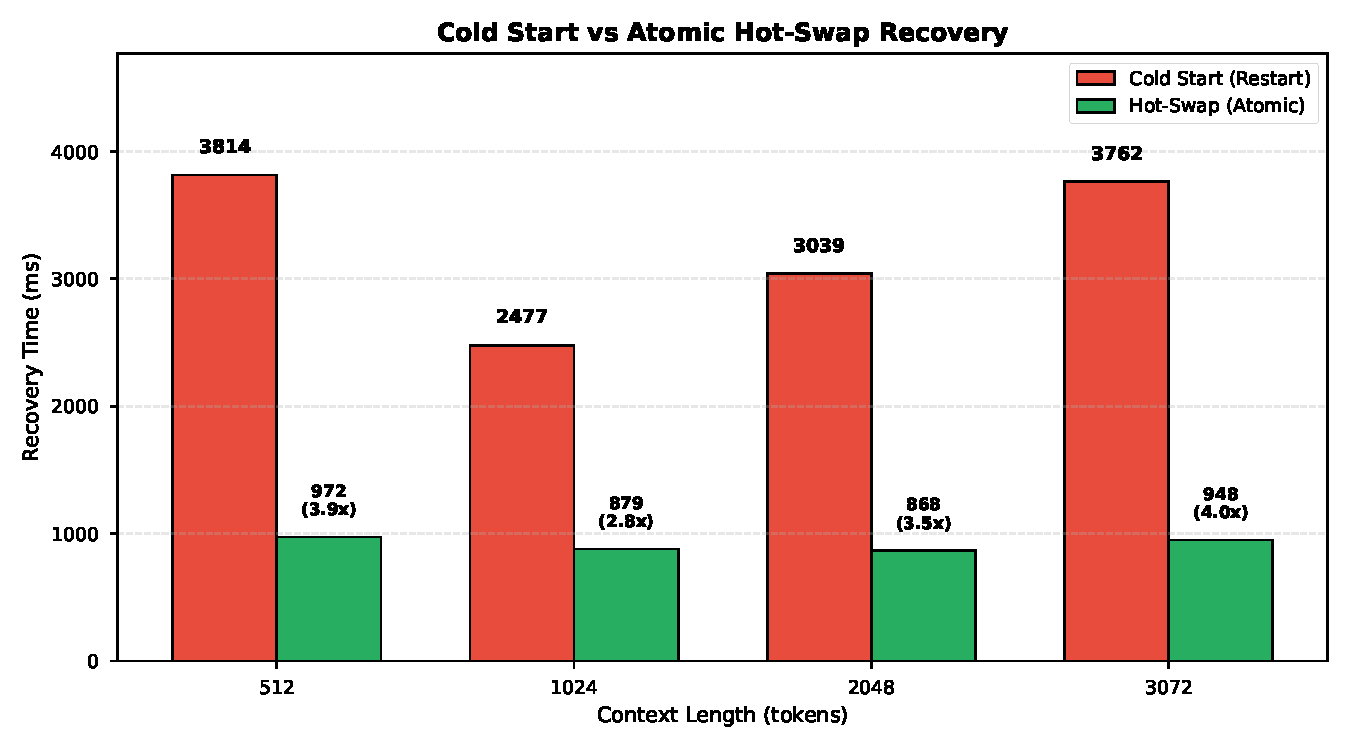
\includegraphics[width=0.96\columnwidth]{figures/01_paper_main/baseline/chart_cold_start_comparison.pdf}
\caption{恢复时延对比：基于重启的恢复 vs. Atomic Hot-Swap。Hot-Swap 在不同上下文规模下实现了 2.8--4.0$\times$ 的加速。}
\label{fig:cold_start}
\end{figure}

\textbf{关键发现}：Atomic Hot-Swap 相比冷重启可实现 \textbf{2.8--4.0$\times$} 更快的恢复。从设计角度看，这说明基于重启的方法会把恢复变成多秒级服务中断，而 EdgeSched 则在后台重载期间维持连续性，并把可见打扰限制在最终切换窗口中。

\subsubsection{作为生命周期鲁棒性的崩溃恢复}

除了迁移行为之外，我们还评估调度器在故障下是否能够正确闭合任务生命周期。因此，我们通过在任务执行过程中随机注入进程崩溃（SIGKILL），测量 \textbf{State Backplane} 的恢复性能。表~\ref{tab:crash_recovery} 给出了崩溃恢复比较结果。

\begin{table}[t]
\centering
\caption{Crash Recovery Comparison}
\label{tab:crash_recovery}
\resizebox{\columnwidth}{!}{%
\begin{tabular}{@{}lccc@{}}
\toprule
\textbf{Metric} & \textbf{Without Backplane} & \textbf{With EdgeSched} & \textbf{Improvement} \\
\midrule
Total Recovery Time (ms) & 7.2 & 44.3 & -- \\
Process Start $\to$ Healthy (ms) & 0.5 & 3.5 & -- \\
Task Recovery Rate & 0\% & \textbf{100\%} & +100\% \\
Tasks Recovered & 0 / 10 & \textbf{10 / 10} & +10 \\
Tasks Lost & 10 & 0 & -100\% \\
\bottomrule
\end{tabular}%
}
\vspace{2pt}
{\small\textit{Note}: Without backplane, process restart is faster but loses all task metadata. With backplane, an additional $\sim$37\,ms buys full semantic recovery.}
\end{table}


\begin{figure}[H]
\centering
\IfFileExists{figures/01_paper_main/robustness/fig_crash_recovery.pdf}{%
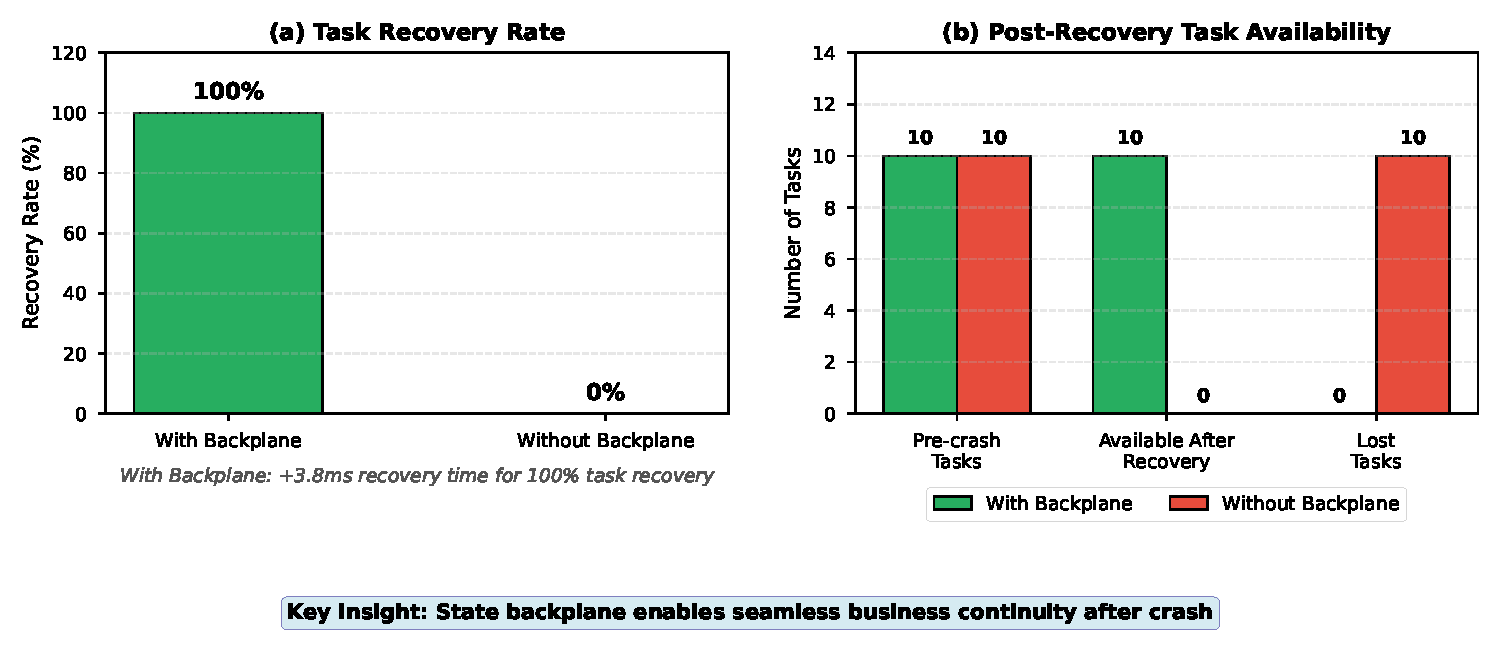
\includegraphics[width=0.96\columnwidth]{figures/01_paper_main/robustness/fig_crash_recovery.pdf}%
}{%
\fbox{\parbox{0.92\columnwidth}{\centering 当前工作区构建中缺少崩溃恢复图。}}%
}
\caption{崩溃恢复对比。没有 backplane 的快速进程重启不会恢复任务元数据，而 EdgeSched 只增加了适度重启开销，便可在语义层面恢复崩溃前的任务集合。}
\label{fig:crash_recovery}
\end{figure}

\textbf{分析}：
\begin{itemize}
\item \textbf{恢复时间}：启用 backplane 后，运行时在我们的测量中可于 44.3 ms 内恢复到语义上可用的状态；相比之下，没有任务恢复能力的纯进程重启为 7.2 ms。
\item \textbf{生命周期闭合}：EdgeSched 能在重启时识别被中断的 ``Running'' 任务，并将其标记为可恢复的失败状态，避免崩溃后积累不一致任务状态。
\item \textbf{恢复开销}：启动额外开销保持在较小水平（约 3 ms），单次状态操作在我们的测量中仍低于 0.01 ms。
\end{itemize}

\subsection{替代设计下的基线行为}

本小节说明保留的基线与本文调度主张之间的关系。

结合表~\ref{tab:cold_start} 中的重启式比较，本文基线覆盖了我们部署类别中的两种实际替代方案：（1）\emph{基于重启的恢复}，通过关闭竞争中的常驻服务并在之后重新加载来解决冲突；（2）\emph{由 OS 管理的内存仲裁}，依赖通用内存管理行为，而不是显式的应用层调度。我们选取这些方案，是因为它们在单台消费级设备上确实是现实选择，即便它们并不实现与 EdgeSched 相同的服务语义。

我们也指出一个重要限制。近年来 LLM 服务文献中存在更强的概念性参照，特别是像 Splitwise、P/D-Serve 和 Inference without Interference 这类相位解耦或干扰感知系统。它们在思想上比本文的实用基线更接近 EdgeSched，但不能直接作为本场景下的实验基线，因为它们针对的是服务器式 LLM 服务栈，而非单机设备上 LLM 服务与图像生成之间的仲裁。因此，我们主要把它们用作定位性参考，并把直接重实现或适配留待未来工作。

\subsubsection{OS 级内存管理（分页/LRU 风格行为）}

我们评估 OS 级内存管理在没有应用层调度的情况下，能否处理多模型并发。该基线代表一种\emph{不带应用层仲裁}的通用内存管理方式：系统依赖 OS 级分页或 LRU 风格行为，而不是显式迁移控制。由于该行为对缓存状态敏感，我们在表~\ref{tab:lru} 中同时报告冷启动与热缓存两种结果。

\begin{table}[H]
\centering
\caption{OS LRU/Unified Memory Baseline (8GB VRAM)}
\label{tab:lru}
\resizebox{\columnwidth}{!}{%
\begin{tabular}{@{}lcc@{}}
\toprule
\textbf{Scenario} & \textbf{Latency (s)} & \textbf{Status} \\
\midrule
LLM Only (cold start, success runs) & 0.41 $\pm$ 0.00 & Normal \\
Image Only (cold start, success runs) & 4.03 $\pm$ 0.03 & Normal \\
Concurrent LLM (cold start) & Timeout ($>$60s) in 1/5 & Unstable / severe thrashing \\
Concurrent LLM (warm cache) & 9.97 $\pm$ 0.06 & $\sim$59.4$\times$ slower \\
Concurrent Image (warm cache) & 2.02 $\pm$ 0.00 & Completed, but LLM degraded \\
\bottomrule
\end{tabular}%
}
\vspace{2pt}
{\small\textit{Note}: In cold-start runs, OS-level LRU/unified-memory behavior timed out in 1 of 5 iterations. In warm-cache runs, image tasks completed, but concurrent LLM latency remained severely inflated relative to LLM-only execution.}
\end{table}


\textbf{关键发现}：在我们的并发工作负载下，OS 级分页/LRU 风格行为变得不可用。在冷启动条件下，5 次迭代中有 1 次在并发执行时超过 60s 超时，表明当两个大模型首次竞争显存时，通用分页行为可能直接失败。在热缓存条件下，图像任务虽然能够完成，但并发 LLM 时延仍上升到 9.97 $\pm$ 0.06 s，约为热缓存下仅运行 LLM 时延 0.168 $\pm$ 0.002 s 的 59.4$\times$。这些结果说明，OS 级内存管理在该场景下缺乏足够可预测性：冷启动可能完全卡死，而热运行也依旧严重退化。

\subsubsection{对称迁移基线}

相对于 EdgeSched 的不对称设计，一个自然替代方案是\textbf{对称迁移}策略，即在两个方向都采用相同的 stop$\rightarrow$migrate$\rightarrow$resume 流程。在这种设计下，上行路径（CPU$\rightarrow$GPU）不会使用后台预加载或原子热切换；相反，它会先停止 CPU 服务，再从头加载 GPU 模型，随后恢复——与下行方向使用的是同一套过程。这个基线很重要，因为它直接检验“单一统一迁移规则”是否能同时适用于两个方向。本文的主张是不能：针对即时资源释放优化的流程，必然暴露可见恢复中断；而针对无缝恢复优化的流程，则必然延迟竞争到来时的资源回收。因此，对称基线隔离出的正是 EdgeSched 的\emph{不对称性为何是必要的}，而不是仅仅“更有好处”。

图~\ref{fig:migration_timeline} 直观展示了两种设计的关键行为差异。在对称情形下（上图），上行恢复需要先停止 CPU 服务，再从头加载 GPU 模型，因此会产生明显的中断窗口；在不对称情形下（下图），CPU 实例在 GPU 实例后台预加载期间继续提供服务，最终原子切换把用户可见中断压缩到接近零。

\begin{figure}[!t]
\centering
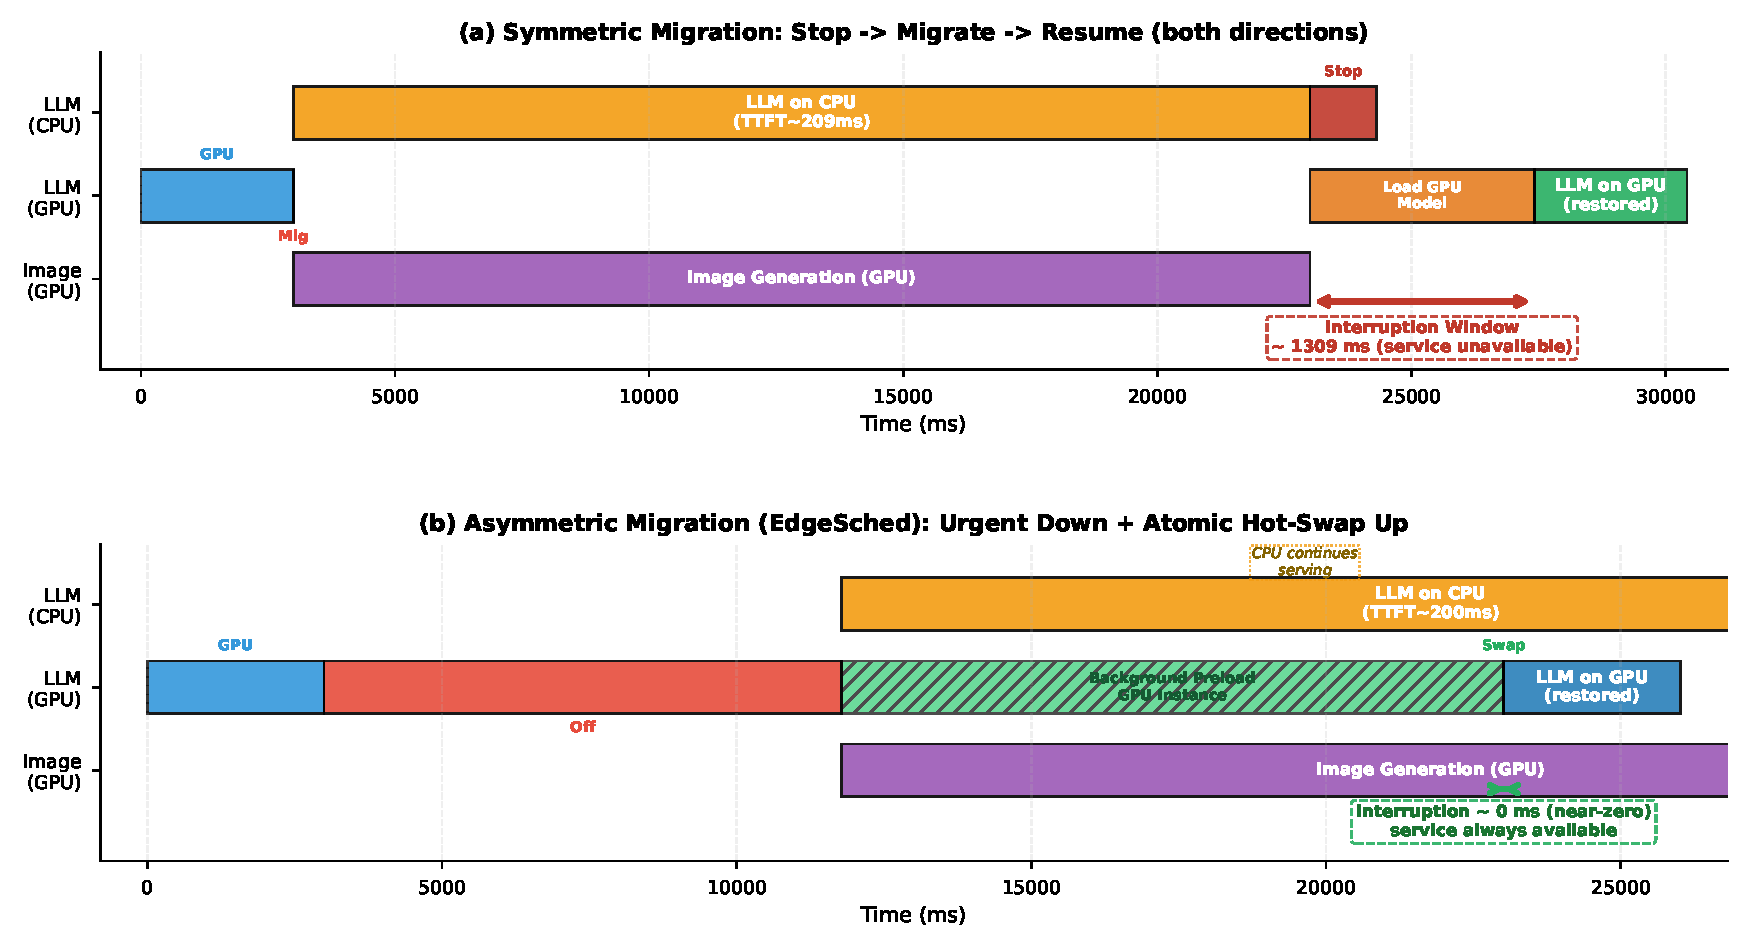
\includegraphics[width=\columnwidth,height=0.17\textheight,keepaspectratio]{figures/01_paper_main/migration/fig_migration_timeline.pdf}
\caption{双面板时间线，对比对称迁移（上）与不对称迁移（EdgeSched，下）。对称设计在上行恢复时存在明显中断窗口，而 EdgeSched 通过后台预加载 GPU 实例，将 Atomic Hot-Swap 的用户感知中断降到接近零。}
\label{fig:migration_timeline}
\end{figure}

表~\ref{tab:migration} 聚焦于两种主要迁移设计。在当前聚合实验中，对称迁移基线在突发工作负载期间可通过 CPU 服务保持共存可用，其 CPU TTFT 为 209.0 $\pm$ 5.7 ms，但由于服务恢复需要经历 stop$\rightarrow$migrate$\rightarrow$resume 切换，其上行中断指标波动很大，达到 1308.9 $\pm$ 2415.0 ms。相比之下，EdgeSched 的 Atomic Hot-Swap 通过在后台预加载 GPU 实例，并让 CPU 实例继续服务请求，把可见中断维持在接近零（$\approx$0 ms）。

\textbf{消融实验}。为了进一步分离两个优化方向的贡献，我们测试了两个消融变体：（1）\emph{Fast-down + naive-up}，在下行路径上使用 EdgeSched 的紧急卸载，但在上行路径上使用朴素的 stop$\rightarrow$migrate$\rightarrow$resume；（2）\emph{Naive-down + optimized-up}，在下行路径上使用朴素卸载，但在上行路径上使用 EdgeSched 的 Atomic Hot-Swap。图~\ref{fig:ablation} 总结了消融结果。上行优化（Atomic Hot-Swap）消除了恢复期间的用户可见中断，而下行优化则相对完整 EdgeSched 路径降低了原始释放时延。把这两点结合起来看，可以清楚说明这两个目标无法由同一个共享过程同时最优达成：快速释放来自更激进的下行处理，而连续性来自延迟切换的上行处理。因此，这两个优化方向共同构成了 EdgeSched 的整体性能特征。

\begin{figure}[!t]
\centering
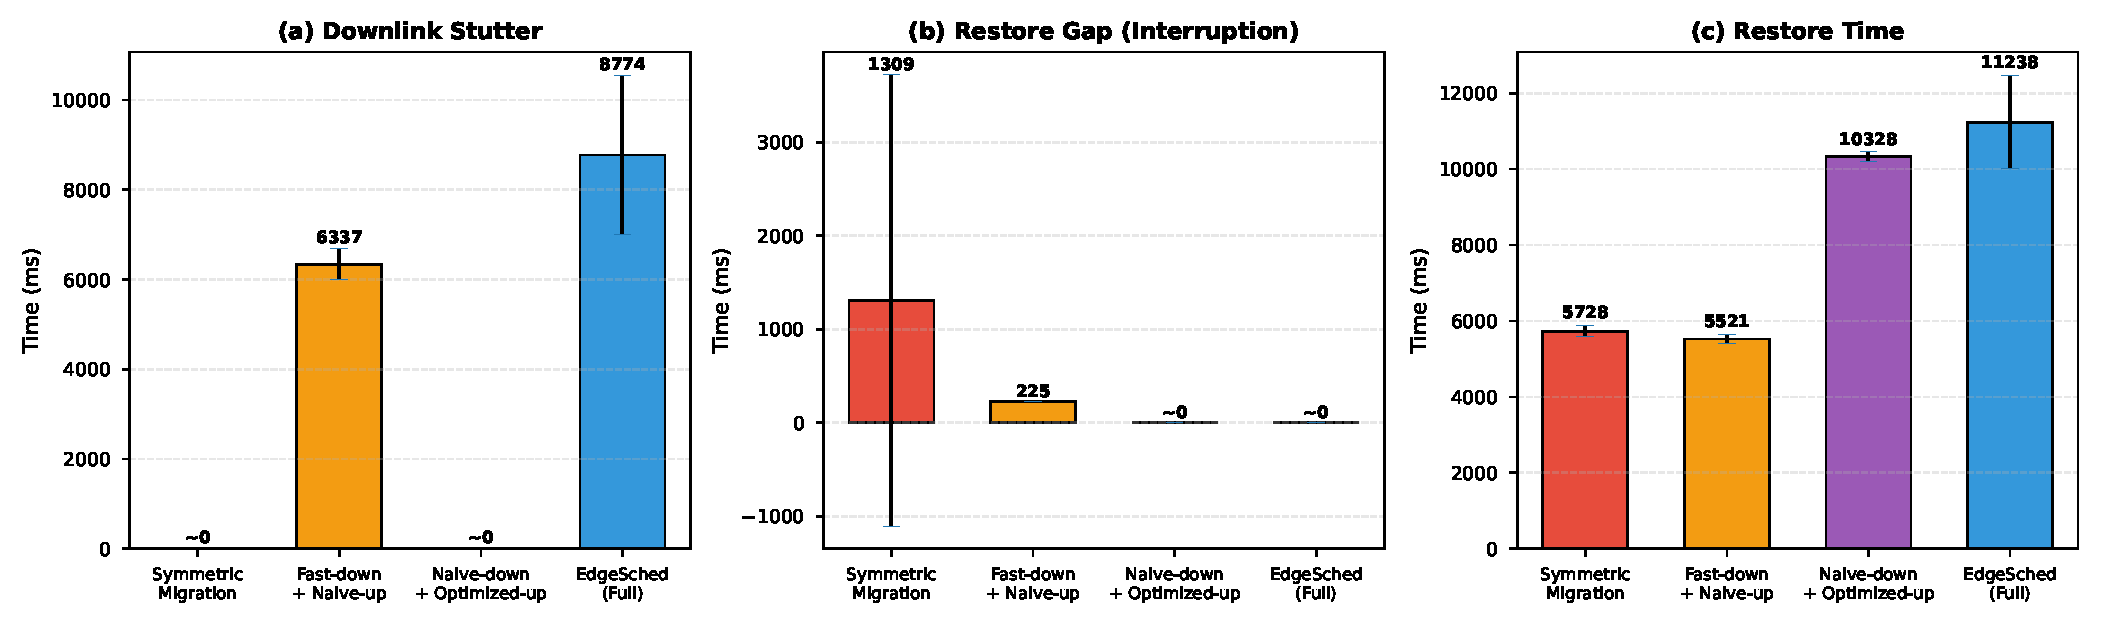
\includegraphics[width=\columnwidth,height=0.17\textheight,keepaspectratio]{figures/01_paper_main/migration/fig_ablation_comparison.pdf}
\caption{四种迁移变体的消融研究。(a)~不同策略下的下行停顿；完整 EdgeSched 路径优先保证安全的分阶段卸载，而不是追求最小原始释放时间。(b)~恢复间隙：只有包含 Atomic Hot-Swap 的变体才能实现接近零的中断。(c)~恢复时间：后台预加载会增加总恢复时间，但把这部分成本隐藏在用户体验之外。}
\label{fig:ablation}
\end{figure}

\subsubsection{操作员管理的手动切换基线}

我们还报告了一个由操作员管理的手动切换基线，用以说明将仲裁推到运行时之外所带来的代价。具体地，操作者使用 llama.cpp 命令行界面（CLI）工具手动卸载常驻模型、运行突发工作负载，再重新加载常驻模型。

\textbf{关键发现}：从手动卸载常驻模型、运行两个图像任务，到重新加载 LLM，整条路径已经需要 \textbf{18.73s}；其中仅 LLM 重载一项（1.49s）在图像生成结束后仍然构成明显恢复成本。我们将这一结果视为证据：外部、由操作员管理的仲裁只适合作为粗粒度兜底方案，而不能替代运行时级调度。

\subsection{吞吐开销与任务成功率}

其余结果用于刻画实现成本及负载下的完成行为。

\textbf{调度器开销}。在一个合成负载微基准测试中（Mock 任务，每轮 $n$=100），相对于原始信号量实现，EdgeSched 的吞吐下降约为 16\%。我们报告这一结果，仅作为实现成本的合理性检查，而非主要调度基线，因为这类方案建模的是通用并发控制，而不是混合工作负载的资源仲裁。

\textbf{压力测试特征}：
\begin{itemize}
\item \textbf{Mock 压力测试}：在仅考察调度器的压力测试中，系统在 200 路并发下完成了全部 2000 个 mock 任务，未观察到失败；在持续 10 分钟的 mock soak 测试中，共处理 5961 个任务，RSS 稳定在约 589 MB（观测范围 586--594 MB）。
\item \textbf{真实混合工作负载压力测试}：在 10 分钟的混合工作负载压力测试（$n$=3）中，EdgeSched 完成了 65/65 个 LLM 请求和 54/54 个图像请求，54/54 次迁移与恢复循环全部成功，且未观察到崩溃。
\item \textbf{真实负载下的时延}：在这些真实压力测试中，聚合后的 LLM TTFT 为 0.95 $\pm$ 0.97 s（最大 3.37 s），图像时延平均为 16.23 $\pm$ 8.49 s。
\item \textbf{开销解释}：相对于原始信号量方案约 16\% 的吞吐下降，反映的是 mock 负载下的实现成本，而非终端用户响应性。在真实混合工作负载中，调度器在保持迁移与恢复正确性的同时，实现了全部请求完成。
\end{itemize}

\begin{figure}[H]
\centering
\IfFileExists{figures/01_paper_main/robustness/fig_stress_test.pdf}{%
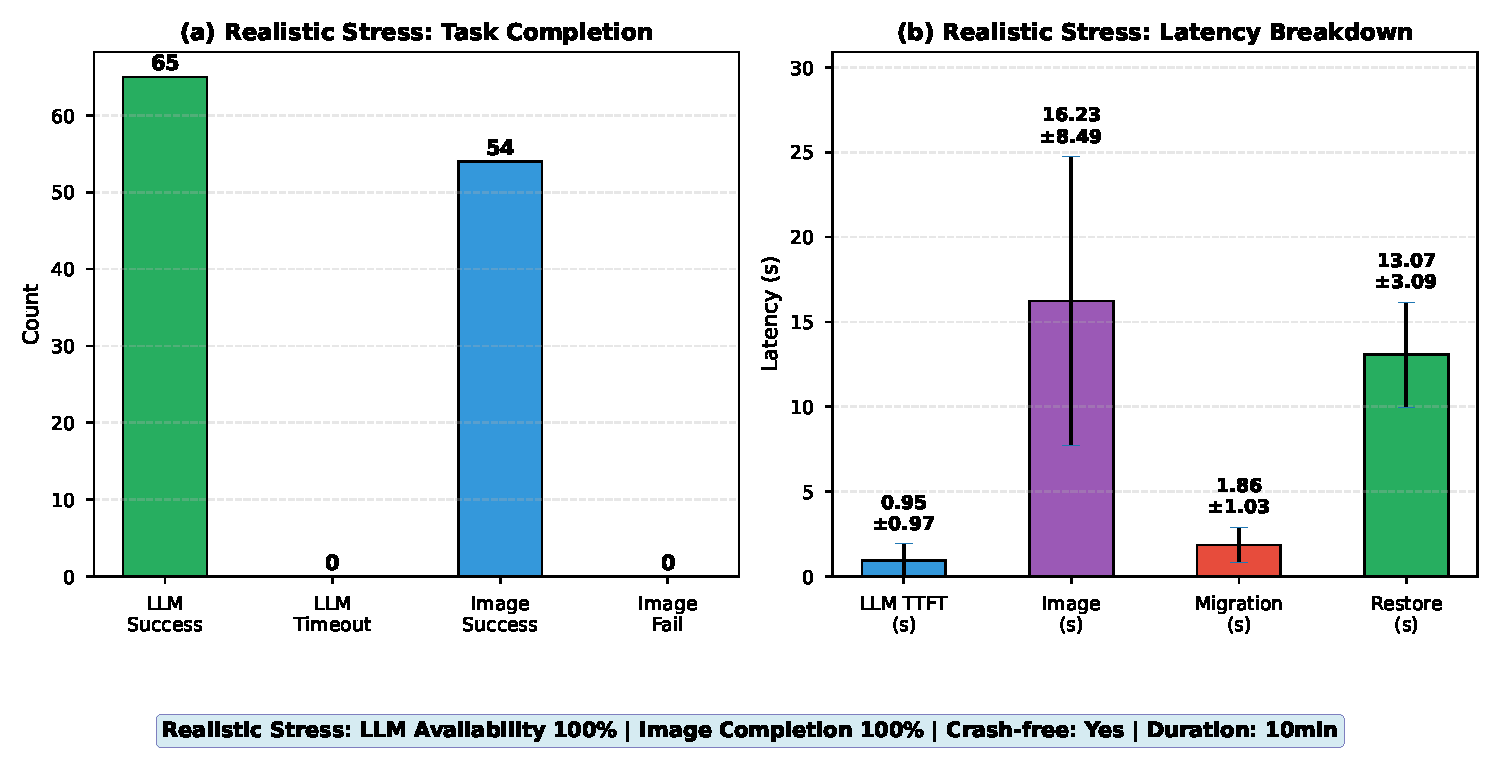
\includegraphics[width=0.96\columnwidth]{figures/01_paper_main/robustness/fig_stress_test.pdf}%
}{%
\fbox{\parbox{0.92\columnwidth}{\centering 当前工作区构建中缺少压力测试图。}}%
}
\caption{10 分钟真实混合工作负载压力测试结果。该图总结了在反复 LLM/图像竞争下的端到端完成情况与时延，显示系统在报告的测试中始终未崩溃，并保持了完整请求完成。}
\label{fig:stress_test}
\end{figure}

\subsection{语义验证}

我们验证了若干调度语义，以支撑前文描述的工作负载抽象和运行时行为。

\begin{enumerate}
\item \textbf{取消}：
\begin{itemize}
\item \textbf{LLM 流式取消}：系统会在下一个协作式取消检查点中途停止生成。
\item \textbf{图像队列取消}：排队中的任务会被立即丢弃；正在运行的任务继续执行，但结果会被丢弃（软取消）。
\end{itemize}

\item \textbf{优先级反转控制}：在我们的混合工作负载测试中，高优先级任务（如用户聊天）会在队列中先于低优先级任务（如后台摘要）被调度。
\end{enumerate}

\subsection{小结}

综合来看，实验表明 EdgeSched 在我们的部署场景中，是 8GB 显存级消费设备上的一个可行设计点。它在 GPU 竞争期间保持常驻服务可达，通过不对称迁移约束恢复成本，在崩溃后约 44 ms 内将任务元数据恢复到语义可用状态，在报告的真实混合工作负载压力测试中维持了全部请求完成，并且相对最小化信号量实现仅引入了适度的 mock 负载吞吐开销（约 16\%）。